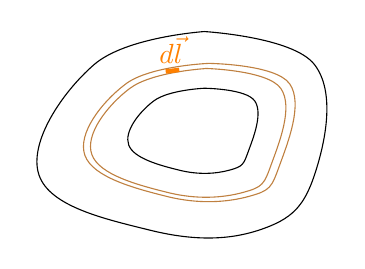
\begin{tikzpicture}
\draw  [scale=1.4] plot[smooth, tension=.7] coordinates {(0,0.8) (-1,0.5) (-1.5,-0.5) (-0.5,-1) (0.5,-1) (1,-0.5) (1,0.5) (0,0.8)};
\draw [scale=0.8]  plot[smooth, tension=.7] coordinates {(0,0.5) (-0.8,0.3) (-1.2,-0.4) (-0.4,-0.8) (0.4,-0.8) (0.7,-0.5) (0.8,0.3) (0,0.5)};
\draw [brown,scale=1.2]  plot[smooth, tension=.7] coordinates {(0.01,0.5412) (-0.7897,0.3308) (-1.1897,-0.3692) (-0.3897,-0.7692) (0.4103,-0.7692) (0.7103,-0.4692) (0.8103,0.3308) (0.0093,0.5431)};
\draw [brown,scale=1.3]  plot[smooth, tension=.7] coordinates {(0.0347,0.55) (-0.7658,0.3508) (-1.1658,-0.3492) (-0.3658,-0.7492) (0.4342,-0.7492) (0.7342,-0.4492) (0.8342,0.3508) (0.0342,0.5508)};

\draw [ultra thick, orange] (-0.4901,0.6125) -- (-0.3177,0.6329);
\node [orange] at (-0.4227,0.8802) {$d\vec{l}$};
\end{tikzpicture}